\documentclass[border=1cm, tikz]{standalone}
\usepackage{tikz}
\usetikzlibrary{arrows,arrows.meta,fit,shapes,decorations.pathmorphing,positioning, calc, intersections}
\usepackage[utf8]{inputenc}
\usepackage[T1]{fontenc}

\pgfdeclarelayer{background}
\pgfsetlayers{background,main}
\begin{document}
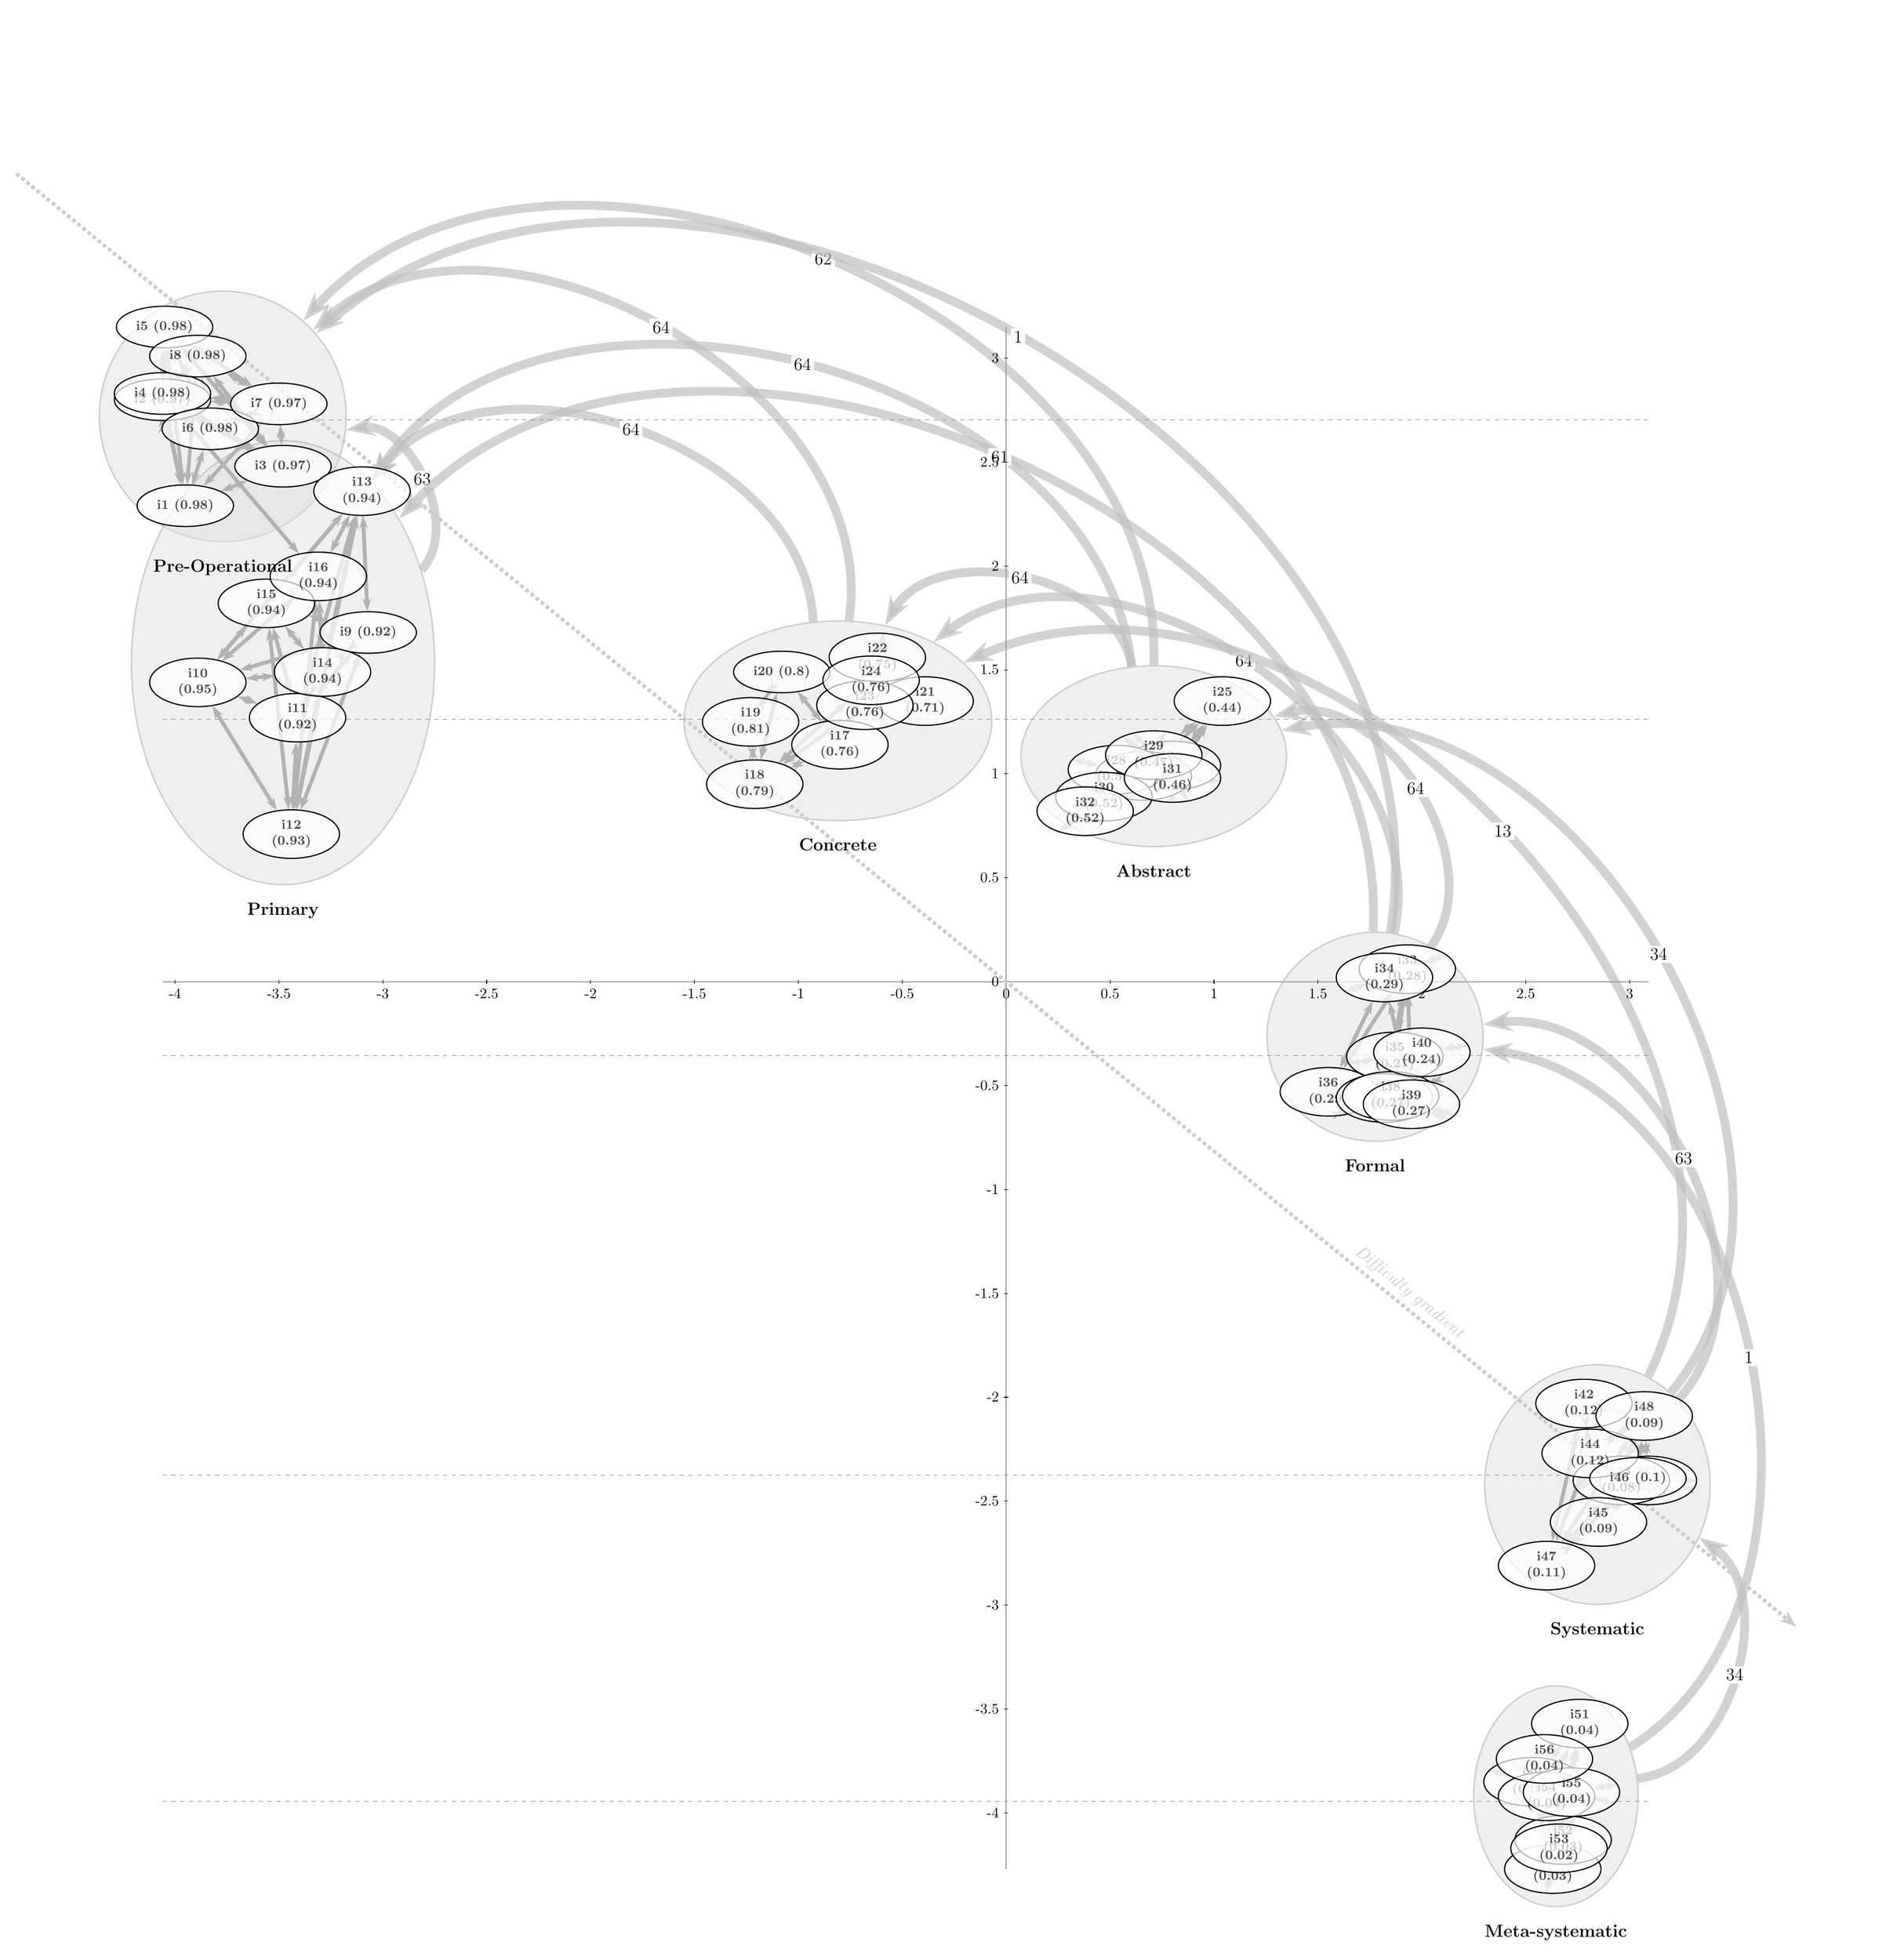
\begin{tikzpicture}[
        scale=5.00,
        thick,
        main node/.style={ellipse, draw, font=\small\bfseries, minimum height=1cm, minimum width=2cm, inner sep=2pt, fill=white, fill opacity=0.7, text width=1.5cm, align=center},
        skill node/.style={circle, fill=gray!75, minimum size=2mm, inner sep=2pt, label={[text width=2.5cm, align=center, text=black!80, font=\large\bfseries, fill=white, fill opacity=0.8,label distance=3mm]above:#1}, fill opacity=1},
        group/.style={draw=gray!50, fill=gray!20, rounded corners=5mm, inner sep=3mm},
        gaussian ellipse/.style={draw=blue!60, fill=blue!10, line width=1pt, opacity=0.7},
        community ellipse/.style={draw=gray!70, fill=lightgray!50, line width=1pt, opacity=0.6},
        auto-ellipse/.style={ellipse, draw=gray!70, fill=lightgray!50, line width=1pt, opacity=0.5, inner sep=0pt},
        arrow/.style={->, -{Stealth[length=3mm, width=2mm]},line width=1.5pt, black!70, opacity=0.90, behind path},
        double arrow/.style={=>, {Stealth[length=3mm, width=2mm]}-{Stealth[length=3mm, width=2mm]}, line width=2.5pt, gray!60, opacity=1.00, behind path},
        meta arrow/.style={->, -{Stealth[length=7mm, width=5mm]}, line width=6pt, gray!50, opacity=0.7, behind path},
        weight label/.style={midway, font=\scriptsize, fill=white, fill opacity=1, text opacity=1, inner sep=2pt, outer sep=0pt, rectangle, draw=none},
        meta label/.style={text=black, midway, font=\large, fill=white, fill opacity=1, text opacity=1, inner sep=2pt, outer sep=0pt, rectangle, draw=none},
        axis style/.style={-, thick, gray!80},
        xtick node/.style={below=0.5mm, font=\small, text=black!60},
        ytick node/.style={left=0.5mm, font=\small, text=black!60}
      ]

% Node definitions
\node[main node] (i1) at (-3.95,2.29) {i1 (0.98)};
\node[main node] (i2) at (-4.06,2.80) {i2 (0.97)};
\node[main node] (i3) at (-3.48,2.48) {i3 (0.97)};
\node[main node] (i4) at (-4.06,2.83) {i4 (0.98)};
\node[main node] (i5) at (-4.05,3.15) {i5 (0.98)};
\node[main node] (i6) at (-3.83,2.66) {i6 (0.98)};
\node[main node] (i7) at (-3.50,2.78) {i7 (0.97)};
\node[main node] (i8) at (-3.89,3.01) {i8 (0.98)};
\node[main node] (i9) at (-3.07,1.68) {i9 (0.92)};
\node[main node] (i10) at (-3.89,1.44) {i10 (0.95)};
\node[main node] (i11) at (-3.41,1.27) {i11 (0.92)};
\node[main node] (i12) at (-3.44,0.71) {i12 (0.93)};
\node[main node] (i13) at (-3.10,2.36) {i13 (0.94)};
\node[main node] (i14) at (-3.29,1.49) {i14 (0.94)};
\node[main node] (i15) at (-3.56,1.82) {i15 (0.94)};
\node[main node] (i16) at (-3.31,1.95) {i16 (0.94)};
\node[main node] (i17) at (-0.80,1.14) {i17 (0.76)};
\node[main node] (i18) at (-1.21,0.95) {i18 (0.79)};
\node[main node] (i19) at (-1.23,1.25) {i19 (0.81)};
\node[main node] (i20) at (-1.08,1.49) {i20 (0.8)};
\node[main node] (i21) at (-0.39,1.35) {i21 (0.71)};
\node[main node] (i22) at (-0.62,1.56) {i22 (0.75)};
\node[main node] (i23) at (-0.68,1.33) {i23 (0.76)};
\node[main node] (i24) at (-0.65,1.45) {i24 (0.76)};
\node[main node] (i25) at (1.04,1.35) {i25 (0.44)};
\node[main node] (i26) at (0.80,1.04) {i26 (0.48)};
\node[main node] (i27) at (0.66,0.99) {i27 (0.47)};
\node[main node] (i28) at (0.53,1.02) {i28 (0.51)};
\node[main node] (i29) at (0.71,1.09) {i29 (0.47)};
\node[main node] (i30) at (0.47,0.89) {i30 (0.52)};
\node[main node] (i31) at (0.80,0.98) {i31 (0.46)};
\node[main node] (i32) at (0.38,0.82) {i32 (0.52)};
\node[main node] (i33) at (1.93,0.06) {i33 (0.28)};
\node[main node] (i34) at (1.82,0.02) {i34 (0.29)};
\node[main node] (i35) at (1.87,-0.36) {i35 (0.27)};
\node[main node] (i36) at (1.55,-0.53) {i36 (0.29)};
\node[main node] (i37) at (1.82,-0.56) {i37 (0.24)};
\node[main node] (i38) at (1.85,-0.55) {i38 (0.27)};
\node[main node] (i39) at (1.95,-0.59) {i39 (0.27)};
\node[main node] (i40) at (2.00,-0.34) {i40 (0.24)};
\node[main node] (i41) at (3.09,-2.40) {i41 (0.08)};
\node[main node] (i42) at (2.78,-2.03) {i42 (0.12)};
\node[main node] (i43) at (2.96,-2.40) {i43 (0.08)};
\node[main node] (i44) at (2.81,-2.27) {i44 (0.12)};
\node[main node] (i45) at (2.85,-2.60) {i45 (0.09)};
\node[main node] (i46) at (3.04,-2.39) {i46 (0.1)};
\node[main node] (i47) at (2.60,-2.81) {i47 (0.11)};
\node[main node] (i48) at (3.07,-2.09) {i48 (0.09)};
\node[main node] (i49) at (2.53,-3.85) {i49 (0.05)};
\node[main node] (i50) at (2.63,-4.27) {i50 (0.03)};
\node[main node] (i51) at (2.76,-3.57) {i51 (0.04)};
\node[main node] (i52) at (2.68,-4.13) {i52 (0.03)};
\node[main node] (i53) at (2.66,-4.17) {i53 (0.02)};
\node[main node] (i54) at (2.60,-3.92) {i54 (0.04)};
\node[main node] (i55) at (2.72,-3.90) {i55 (0.04)};
\node[main node] (i56) at (2.59,-3.74) {i56 (0.04)};

\begin{pgfonlayer}{background}
% Gaussian ellipses for communities
\node[auto-ellipse, fit=(i1) (i2) (i3) (i4) (i5) (i6) (i7) (i8), scale=0.80] (Cluster1) {};
\node[auto-ellipse, fit=(i9) (i10) (i11) (i12) (i13) (i14) (i15) (i16), scale=0.80] (Cluster2) {};
\node[auto-ellipse, fit=(i17) (i18) (i19) (i20) (i21) (i22) (i23) (i24), scale=0.80] (Cluster3) {};
\node[auto-ellipse, fit=(i25) (i26) (i27) (i28) (i29) (i30) (i31) (i32), scale=0.80] (Cluster4) {};
\node[auto-ellipse, fit=(i33) (i34) (i35) (i36) (i37) (i38) (i39) (i40), scale=0.80] (Cluster5) {};
\node[auto-ellipse, fit=(i41) (i42) (i43) (i44) (i45) (i46) (i47) (i48), scale=0.80] (Cluster6) {};
\node[auto-ellipse, fit=(i49) (i50) (i51) (i52) (i53) (i54) (i55) (i56), scale=0.80] (Cluster7) {};

% Metagraph
\draw[meta arrow, bend right=70] (Cluster2) to[bend right] (Cluster1);
\path (Cluster2) to[bend right=70] node[meta label] {63} (Cluster1);
\draw[meta arrow, bend right=70] (Cluster3) to[bend right] (Cluster1);
\path (Cluster3) to[bend right=70] node[meta label] {64} (Cluster1);
\draw[meta arrow, bend right=70] (Cluster3) to[bend right] (Cluster2);
\path (Cluster3) to[bend right=70] node[meta label] {64} (Cluster2);
\draw[meta arrow, bend right=70] (Cluster4) to[bend right] (Cluster1);
\path (Cluster4) to[bend right=70] node[meta label] {62} (Cluster1);
\draw[meta arrow, bend right=70] (Cluster4) to[bend right] (Cluster2);
\path (Cluster4) to[bend right=70] node[meta label] {64} (Cluster2);
\draw[meta arrow, bend right=70] (Cluster4) to[bend right] (Cluster3);
\path (Cluster4) to[bend right=70] node[meta label] {64} (Cluster3);
\draw[meta arrow, bend right=70] (Cluster5) to[bend right] (Cluster1);
\path (Cluster5) to[bend right=70] node[meta label] {1} (Cluster1);
\draw[meta arrow, bend right=70] (Cluster5) to[bend right] (Cluster2);
\path (Cluster5) to[bend right=70] node[meta label] {61} (Cluster2);
\draw[meta arrow, bend right=70] (Cluster5) to[bend right] (Cluster3);
\path (Cluster5) to[bend right=70] node[meta label] {64} (Cluster3);
\draw[meta arrow, bend right=70] (Cluster5) to[bend right] (Cluster4);
\path (Cluster5) to[bend right=70] node[meta label] {64} (Cluster4);
\draw[meta arrow, bend right=70] (Cluster6) to[bend right] (Cluster3);
\path (Cluster6) to[bend right=70] node[meta label] {13} (Cluster3);
\draw[meta arrow, bend right=70] (Cluster6) to[bend right] (Cluster4);
\path (Cluster6) to[bend right=70] node[meta label] {34} (Cluster4);
\draw[meta arrow, bend right=70] (Cluster6) to[bend right] (Cluster5);
\path (Cluster6) to[bend right=70] node[meta label] {63} (Cluster5);
\draw[meta arrow, bend right=70] (Cluster7) to[bend right] (Cluster5);
\path (Cluster7) to[bend right=70] node[meta label] {1} (Cluster5);
\draw[meta arrow, bend right=70] (Cluster7) to[bend right] (Cluster6);
\path (Cluster7) to[bend right=70] node[meta label] {34} (Cluster6);

% Axes
\draw[axis style] (-4.06,0) -- (3.09,0);
\draw[axis style] (0,-4.27) -- (0,3.15);

% Axis ticks
\foreach \x in {-4,-3.5,-3,-2.5,-2,-1.5,-1,-0.5,0,0.5,1,1.5,2,2.5,3}
  {\draw (\x,-0.01) -- (\x,0.01); \node[below] at (\x,-0.01) {\x};}
\foreach \y in {-4,-3.5,-3,-2.5,-2,-1.5,-1,-0.5,0,0.5,1,1.5,2,2.5,3}
  {\draw (-0.01,\y) -- (0.01,\y); \node[left] at (-0.01,\y) {\y};}


% Difficulty gradient line
\draw[gray!40, line width=2.5pt, dotted, -{Stealth[length=4mm, width=3mm]}] (-4.7628,3.8876) -- (3.8016,-3.1031);
\node[rotate=320.8, font=\large\itshape, text=gray!40, above=1pt] at (1.9008,-1.5515) {Difficulty gradient};

% logOR level lines
\draw[gray, dashed] (-4.06,-3.9439) -- (3.09,-3.9439);
\draw[gray, dashed] (-4.06,-2.3747) -- (3.09,-2.3747);
\draw[gray, dashed] (-4.06,-0.3556) -- (3.09,-0.3556);
\draw[gray, dashed] (-4.06,1.2635) -- (3.09,1.2635);
\draw[gray, dashed] (-4.06,2.7038) -- (3.09,2.7038);

% Symmetric association links
\draw[double arrow] (i2) to (i1);
\draw[double arrow] (i2) to (i3);
\draw[double arrow] (i2) to (i4);
\draw[double arrow] (i2) to (i5);
\draw[double arrow] (i2) to (i6);
\draw[double arrow] (i2) to (i7);
\draw[double arrow] (i2) to (i8);
\draw[double arrow] (i3) to (i1);
\draw[double arrow] (i3) to (i2);
\draw[double arrow] (i3) to (i4);
\draw[double arrow] (i3) to (i5);
\draw[double arrow] (i3) to (i6);
\draw[double arrow] (i3) to (i7);
\draw[double arrow] (i3) to (i8);
\draw[double arrow] (i4) to (i1);
\draw[double arrow] (i4) to (i2);
\draw[double arrow] (i4) to (i3);
\draw[double arrow] (i4) to (i5);
\draw[double arrow] (i4) to (i6);
\draw[double arrow] (i4) to (i7);
\draw[double arrow] (i4) to (i8);
\draw[double arrow] (i4) to (i16);
\draw[double arrow] (i5) to (i1);
\draw[double arrow] (i5) to (i2);
\draw[double arrow] (i5) to (i3);
\draw[double arrow] (i5) to (i4);
\draw[double arrow] (i5) to (i6);
\draw[double arrow] (i5) to (i7);
\draw[double arrow] (i5) to (i8);
\draw[double arrow] (i6) to (i1);
\draw[double arrow] (i6) to (i2);
\draw[double arrow] (i6) to (i3);
\draw[double arrow] (i6) to (i4);
\draw[double arrow] (i6) to (i5);
\draw[double arrow] (i6) to (i7);
\draw[double arrow] (i6) to (i8);
\draw[double arrow] (i7) to (i1);
\draw[double arrow] (i7) to (i2);
\draw[double arrow] (i7) to (i3);
\draw[double arrow] (i7) to (i4);
\draw[double arrow] (i7) to (i5);
\draw[double arrow] (i7) to (i6);
\draw[double arrow] (i7) to (i8);
\draw[double arrow] (i8) to (i1);
\draw[double arrow] (i8) to (i2);
\draw[double arrow] (i8) to (i3);
\draw[double arrow] (i8) to (i4);
\draw[double arrow] (i8) to (i5);
\draw[double arrow] (i8) to (i6);
\draw[double arrow] (i8) to (i7);
\draw[double arrow] (i9) to (i10);
\draw[double arrow] (i9) to (i11);
\draw[double arrow] (i9) to (i12);
\draw[double arrow] (i9) to (i13);
\draw[double arrow] (i9) to (i14);
\draw[double arrow] (i9) to (i15);
\draw[double arrow] (i10) to (i9);
\draw[double arrow] (i10) to (i11);
\draw[double arrow] (i10) to (i12);
\draw[double arrow] (i10) to (i13);
\draw[double arrow] (i10) to (i14);
\draw[double arrow] (i10) to (i15);
\draw[double arrow] (i10) to (i16);
\draw[double arrow] (i11) to (i9);
\draw[double arrow] (i11) to (i10);
\draw[double arrow] (i11) to (i12);
\draw[double arrow] (i11) to (i13);
\draw[double arrow] (i11) to (i14);
\draw[double arrow] (i11) to (i15);
\draw[double arrow] (i12) to (i9);
\draw[double arrow] (i12) to (i10);
\draw[double arrow] (i12) to (i11);
\draw[double arrow] (i12) to (i13);
\draw[double arrow] (i12) to (i14);
\draw[double arrow] (i12) to (i15);
\draw[double arrow] (i12) to (i16);
\draw[double arrow] (i13) to (i9);
\draw[double arrow] (i13) to (i10);
\draw[double arrow] (i13) to (i11);
\draw[double arrow] (i13) to (i12);
\draw[double arrow] (i13) to (i14);
\draw[double arrow] (i13) to (i15);
\draw[double arrow] (i13) to (i16);
\draw[double arrow] (i14) to (i9);
\draw[double arrow] (i14) to (i10);
\draw[double arrow] (i14) to (i11);
\draw[double arrow] (i14) to (i12);
\draw[double arrow] (i14) to (i13);
\draw[double arrow] (i14) to (i15);
\draw[double arrow] (i14) to (i16);
\draw[double arrow] (i15) to (i9);
\draw[double arrow] (i15) to (i10);
\draw[double arrow] (i15) to (i11);
\draw[double arrow] (i15) to (i12);
\draw[double arrow] (i15) to (i13);
\draw[double arrow] (i15) to (i14);
\draw[double arrow] (i15) to (i16);
\draw[double arrow] (i16) to (i4);
\draw[double arrow] (i16) to (i10);
\draw[double arrow] (i16) to (i12);
\draw[double arrow] (i16) to (i13);
\draw[double arrow] (i16) to (i14);
\draw[double arrow] (i16) to (i15);
\draw[double arrow] (i17) to (i18);
\draw[double arrow] (i17) to (i20);
\draw[double arrow] (i17) to (i22);
\draw[double arrow] (i17) to (i23);
\draw[double arrow] (i17) to (i24);
\draw[double arrow] (i18) to (i17);
\draw[double arrow] (i18) to (i19);
\draw[double arrow] (i18) to (i20);
\draw[double arrow] (i18) to (i23);
\draw[double arrow] (i18) to (i24);
\draw[double arrow] (i19) to (i18);
\draw[double arrow] (i19) to (i20);
\draw[double arrow] (i20) to (i17);
\draw[double arrow] (i20) to (i18);
\draw[double arrow] (i20) to (i19);
\draw[double arrow] (i22) to (i17);
\draw[double arrow] (i22) to (i23);
\draw[double arrow] (i22) to (i24);
\draw[double arrow] (i23) to (i17);
\draw[double arrow] (i23) to (i18);
\draw[double arrow] (i23) to (i22);
\draw[double arrow] (i23) to (i24);
\draw[double arrow] (i24) to (i17);
\draw[double arrow] (i24) to (i18);
\draw[double arrow] (i24) to (i22);
\draw[double arrow] (i24) to (i23);
\draw[double arrow] (i25) to (i26);
\draw[double arrow] (i25) to (i27);
\draw[double arrow] (i25) to (i29);
\draw[double arrow] (i25) to (i31);
\draw[double arrow] (i26) to (i25);
\draw[double arrow] (i26) to (i27);
\draw[double arrow] (i26) to (i28);
\draw[double arrow] (i26) to (i29);
\draw[double arrow] (i26) to (i31);
\draw[double arrow] (i27) to (i25);
\draw[double arrow] (i27) to (i26);
\draw[double arrow] (i27) to (i28);
\draw[double arrow] (i27) to (i29);
\draw[double arrow] (i27) to (i30);
\draw[double arrow] (i27) to (i31);
\draw[double arrow] (i27) to (i32);
\draw[double arrow] (i28) to (i26);
\draw[double arrow] (i28) to (i27);
\draw[double arrow] (i28) to (i29);
\draw[double arrow] (i28) to (i30);
\draw[double arrow] (i28) to (i31);
\draw[double arrow] (i28) to (i32);
\draw[double arrow] (i29) to (i25);
\draw[double arrow] (i29) to (i26);
\draw[double arrow] (i29) to (i27);
\draw[double arrow] (i29) to (i28);
\draw[double arrow] (i29) to (i31);
\draw[double arrow] (i29) to (i32);
\draw[double arrow] (i30) to (i27);
\draw[double arrow] (i30) to (i28);
\draw[double arrow] (i30) to (i31);
\draw[double arrow] (i30) to (i32);
\draw[double arrow] (i31) to (i25);
\draw[double arrow] (i31) to (i26);
\draw[double arrow] (i31) to (i27);
\draw[double arrow] (i31) to (i28);
\draw[double arrow] (i31) to (i29);
\draw[double arrow] (i31) to (i30);
\draw[double arrow] (i32) to (i27);
\draw[double arrow] (i32) to (i28);
\draw[double arrow] (i32) to (i29);
\draw[double arrow] (i32) to (i30);
\draw[double arrow] (i33) to (i34);
\draw[double arrow] (i33) to (i35);
\draw[double arrow] (i33) to (i36);
\draw[double arrow] (i33) to (i37);
\draw[double arrow] (i33) to (i38);
\draw[double arrow] (i33) to (i39);
\draw[double arrow] (i34) to (i33);
\draw[double arrow] (i34) to (i36);
\draw[double arrow] (i34) to (i39);
\draw[double arrow] (i35) to (i33);
\draw[double arrow] (i35) to (i37);
\draw[double arrow] (i35) to (i38);
\draw[double arrow] (i35) to (i39);
\draw[double arrow] (i35) to (i40);
\draw[double arrow] (i36) to (i33);
\draw[double arrow] (i36) to (i34);
\draw[double arrow] (i37) to (i33);
\draw[double arrow] (i37) to (i35);
\draw[double arrow] (i37) to (i38);
\draw[double arrow] (i37) to (i39);
\draw[double arrow] (i37) to (i40);
\draw[double arrow] (i38) to (i33);
\draw[double arrow] (i38) to (i35);
\draw[double arrow] (i38) to (i37);
\draw[double arrow] (i38) to (i39);
\draw[double arrow] (i39) to (i33);
\draw[double arrow] (i39) to (i34);
\draw[double arrow] (i39) to (i35);
\draw[double arrow] (i39) to (i37);
\draw[double arrow] (i39) to (i38);
\draw[double arrow] (i39) to (i40);
\draw[double arrow] (i40) to (i35);
\draw[double arrow] (i40) to (i37);
\draw[double arrow] (i40) to (i39);
\draw[double arrow] (i41) to (i43);
\draw[double arrow] (i41) to (i45);
\draw[double arrow] (i41) to (i46);
\draw[double arrow] (i41) to (i48);
\draw[double arrow] (i42) to (i44);
\draw[double arrow] (i42) to (i47);
\draw[double arrow] (i42) to (i48);
\draw[double arrow] (i43) to (i41);
\draw[double arrow] (i43) to (i45);
\draw[double arrow] (i43) to (i46);
\draw[double arrow] (i43) to (i47);
\draw[double arrow] (i43) to (i48);
\draw[double arrow] (i44) to (i42);
\draw[double arrow] (i44) to (i46);
\draw[double arrow] (i44) to (i47);
\draw[double arrow] (i44) to (i48);
\draw[double arrow] (i45) to (i41);
\draw[double arrow] (i45) to (i43);
\draw[double arrow] (i45) to (i46);
\draw[double arrow] (i45) to (i47);
\draw[double arrow] (i45) to (i48);
\draw[double arrow] (i46) to (i41);
\draw[double arrow] (i46) to (i43);
\draw[double arrow] (i46) to (i44);
\draw[double arrow] (i46) to (i45);
\draw[double arrow] (i46) to (i47);
\draw[double arrow] (i46) to (i48);
\draw[double arrow] (i47) to (i42);
\draw[double arrow] (i47) to (i43);
\draw[double arrow] (i47) to (i44);
\draw[double arrow] (i47) to (i45);
\draw[double arrow] (i47) to (i46);
\draw[double arrow] (i47) to (i48);
\draw[double arrow] (i48) to (i41);
\draw[double arrow] (i48) to (i42);
\draw[double arrow] (i48) to (i43);
\draw[double arrow] (i48) to (i44);
\draw[double arrow] (i48) to (i45);
\draw[double arrow] (i48) to (i46);
\draw[double arrow] (i48) to (i47);
\draw[double arrow] (i49) to (i50);
\draw[double arrow] (i49) to (i51);
\draw[double arrow] (i49) to (i52);
\draw[double arrow] (i49) to (i53);
\draw[double arrow] (i49) to (i54);
\draw[double arrow] (i49) to (i55);
\draw[double arrow] (i50) to (i49);
\draw[double arrow] (i50) to (i51);
\draw[double arrow] (i50) to (i52);
\draw[double arrow] (i50) to (i53);
\draw[double arrow] (i50) to (i54);
\draw[double arrow] (i50) to (i55);
\draw[double arrow] (i51) to (i49);
\draw[double arrow] (i51) to (i50);
\draw[double arrow] (i51) to (i53);
\draw[double arrow] (i51) to (i54);
\draw[double arrow] (i51) to (i55);
\draw[double arrow] (i52) to (i49);
\draw[double arrow] (i52) to (i50);
\draw[double arrow] (i52) to (i53);
\draw[double arrow] (i52) to (i54);
\draw[double arrow] (i52) to (i55);
\draw[double arrow] (i53) to (i49);
\draw[double arrow] (i53) to (i50);
\draw[double arrow] (i53) to (i51);
\draw[double arrow] (i53) to (i52);
\draw[double arrow] (i53) to (i54);
\draw[double arrow] (i53) to (i55);
\draw[double arrow] (i54) to (i49);
\draw[double arrow] (i54) to (i50);
\draw[double arrow] (i54) to (i51);
\draw[double arrow] (i54) to (i52);
\draw[double arrow] (i54) to (i53);
\draw[double arrow] (i54) to (i55);
\draw[double arrow] (i55) to (i49);
\draw[double arrow] (i55) to (i50);
\draw[double arrow] (i55) to (i51);
\draw[double arrow] (i55) to (i52);
\draw[double arrow] (i55) to (i53);
\draw[double arrow] (i55) to (i54);
\draw[double arrow] (i56) to (i49);
\draw[double arrow] (i56) to (i50);
\draw[double arrow] (i56) to (i51);
\draw[double arrow] (i56) to (i52);
\draw[double arrow] (i56) to (i53);
\draw[double arrow] (i56) to (i54);
\draw[double arrow] (i56) to (i55);
\end{pgfonlayer}

% Cluster labels (foreground)
\node[font=\large\bfseries, below=3mm] at (Cluster1.south) {Pre-Operational};
\node[font=\large\bfseries, below=3mm] at (Cluster2.south) {Primary};
\node[font=\large\bfseries, below=3mm] at (Cluster3.south) {Concrete};
\node[font=\large\bfseries, below=3mm] at (Cluster4.south) {Abstract};
\node[font=\large\bfseries, below=3mm] at (Cluster5.south) {Formal};
\node[font=\large\bfseries, below=3mm] at (Cluster6.south) {Systematic};
\node[font=\large\bfseries, below=3mm] at (Cluster7.south) {Meta-systematic};

\end{tikzpicture}
\end{document}
